\documentclass[tikz, convert = false]{standalone}%

\usepackage[utf8]{inputenx}%  http://ctan.org/pkg/inputenx
% Euler for math | Palatino for rm | Helvetica for ss | Courier for tt
\renewcommand{\rmdefault}{ppl}% rm
\linespread{1.05}% Palatino needs more leading
\usepackage[scaled]{helvet}% ss //  http://ctan.org/pkg/helvet
\usepackage{courier}% tt // http://ctan.org/pkg/courier
\usepackage{eulervm}  %  http://ctan.org/pkg/eulervm
% a better implementation of the euler package (not in gwTeX)
\normalfont%
\usepackage[T1]{fontenc}%  http://ctan.org/pkg/fontenc
\usepackage{textcomp}%  http://ctan.org/pkg/textcomp

\usepackage{pgfplots}
\pgfplotsset{compat = 1.10}

\begin{document}
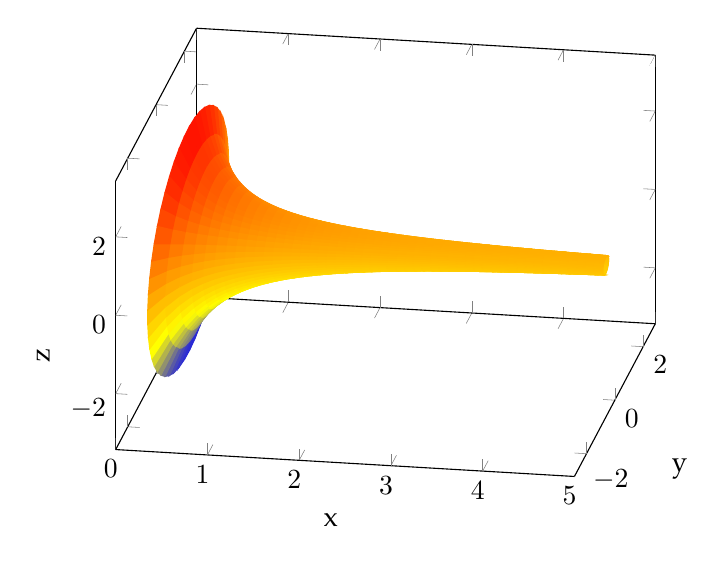
\begin{tikzpicture}
  \begin{axis}[
    no marks,
    view = {10}{30},
    xmin = 0,
    xmax = 5,
    xlabel = {x},
    ylabel = {y},
    zlabel = {z}
    ]
    \addplot3[surf, shader = flat, samples = 50, domain = 0.35:4.9,
    y domain = 0:2*pi, z buffer = sort]
    (x, {(1/x)*cos(deg(y))}, {(1/x)*sin(deg(y))});
  \end{axis}
\end{tikzpicture}
\end{document}
%%% Local Variables:
%%% mode: latex
%%% TeX-master: t
%%% End:
